\documentclass[12pt]{article}

\usepackage{fullpage}
\usepackage{datetime}
\usepackage{amsfonts}
\usepackage{amsmath}

\usepackage{graphicx}
\usepackage{subcaption}

\usepackage{biblatex}
\addbibresource{./references.bib}

\title{
  Learning Neural Orientation Field for Volumetric Hair Reconstruction \\
  {
    \small
    Project Milestone
  }
}
\author{
  Fangjun Zhou \\ fzhou48
  \and Weiran Xu \\ weiran
  \and Zhenyu Zhang \\ zhenyuz5
}
\date{\today}

\begin{document}
  \maketitle

  \section{Introduction}
  % Project motivation

  Reconstructing human hair is one of the most challenging yet critical process in rendering photorealistic digital human. Unlike other parts of the human body, human hair is highly detailed and often intertwined together. Therefore, it's difficult to use traditional photogrammetry method to reconstruct its structure.

  Before machine learning model is used in this field, artists often hand crafted splines on skulls to represent hair strands. Each strand is then textured and rendered to mimic the hair volume. This workflow requires a lot of experience as it's non-trivial for artists to infer the final render result from hair stand splines. To reduce the workload and improve the accuracy of hair reconstruction, machine learning models are trained to generate hair strand from captured images.

  In this work, we propose a new method capturing the hair structure by a 3D orientation field from $\mathbb{R}^{3} \rightarrow \mathbb{R}^{2}$ representing the hair growing direction and occupancy. On top of that, another occupancy field from $\mathbb{R}^{3} \rightarrow \mathbb{R}^{3}$ is learned to indicate void, body, or hair occupancy. These mappings can be used later to generate hair stand directly by numerically solving the PDE. It can also be used as a latent variable to guide other generative models as mentioned in \cite{metzer_latent-nerf_2022}. We can fit this orientation field by a simple MLP. We then project the orientation field onto multiple camera view with a volumetric renderer. Since the screen space projection and volumetric rendering algorithm are differentiable, we are able to learn the orientation field from images from multiple camera angle.

  \section{Related Work}

  Previous attempt to achieve this goal mainly focus on learning based hair strand generation. This includes some studies about single view hair synthesis \cite{saito_3d_2018, zheng_hairstep_2023, wu_neuralhdhair_2022, ma_single-view_nodate}. Since the image only contains hair structure from one viewing angle, it's impossible to reconstruct entire hair accurately. These models often use pretrained image encoders such as ResNet-50 \cite{saito_3d_2018} to encode the abstract hair style into a feature vector, then use generative models such as U-Net \cite{zheng_hairstep_2023}, VAE \cite{saito_3d_2018}, and diffusion models \cite{sklyarova_neural_2023} to generate the final strand. These models also struggle with generating curly hair as there's only limited information about growing direction after feature extraction.

  In \cite{sklyarova_neural_2023} and \cite{rosu_neural_2022}, the authors also tried hair syntheses from multi-view images. However, these two studies still failed to capture finer detail.

  Another study about this topic tried to tackle this problem by expanding the traditional PatchMatch MVS (PMVS) algorithm to a Line-based PatchMatch MVS (LPMVS) \cite{nam_strand-accurate_nodate}. This method, despite its high accuracy, doesn't capture the volumetric property of human hair.

  Our work is highly inspired by NeRF \cite{mildenhall_nerf_2020}, a model used for 3D reconstruction from 2D images. However, our model differs in two major way.

  In NeRF, the model fits a radiance field from $\mathbb{R}^{5} \rightarrow \mathbb{R}^{4}$. The input of the randiance function includes the sample position and view direction. However, since the orientation field our model fits is view-independent, the input space is only $\mathbb{R}^{5}$. This makes it easier for the model to capture more information from a smaller dataset.

  On top of that, the volumetric renderer on orientation field also differs from the one on radiance field. In this case, NeRF only integrate the sampled radiance for each ray, while our model need to project the sample orientation onto the filming plane an then integrate the projected orientation.

  \section{Method}
    \subsection{Data Preprocess}
    
    Our model will be trained on a set of images of human bust from multiple viewing angles.

    $\mathbf{Image:}$  For each of the images, the preprocessing kernel will extract the projection of the hair growing direction onto the camera viewing plane. In this paper, we utilize the preprocessing pipeline in HairStep \cite{zheng_hairstep_2023} to segment out the hair from the image and get the direction vector field of the top layer hair. Each pixel in the preprocessed image has three channels rgb, we use r channel = 255 to denote the pixel belongs to the hair region, and the g and b channel together as the direction vector. For the region that does not belongs to hair but belongs to human body, its rgb = (127, 0, 0), and for other region we set rgb to $\mathbf{0}$.
    \begin{figure}[h]
        \centering
        % first col
        \begin{subfigure}{0.3\textwidth}
            \centering
            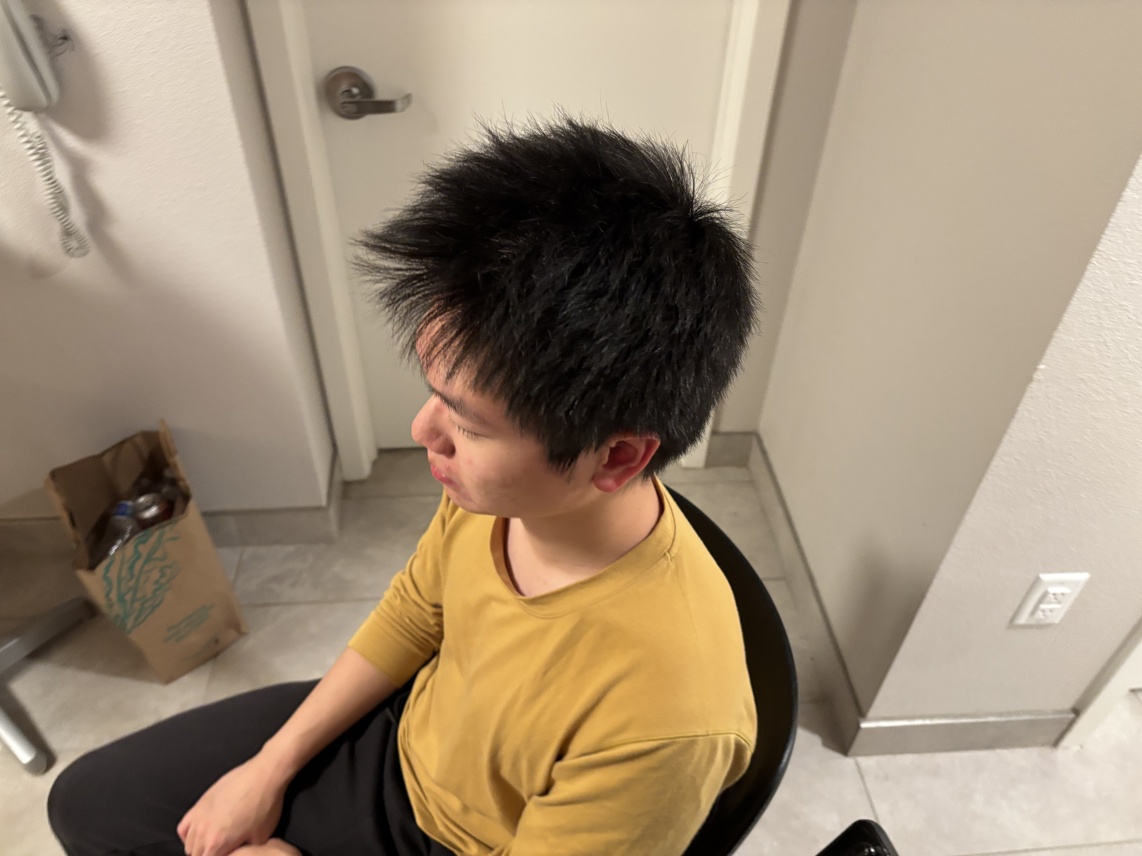
\includegraphics[width=\textwidth]{project-milestone/images/portrait_raw/IMG_0342.png}
            \caption{raw}
        \end{subfigure}
        \hfill
        \begin{subfigure}{0.3\textwidth}
            \centering
            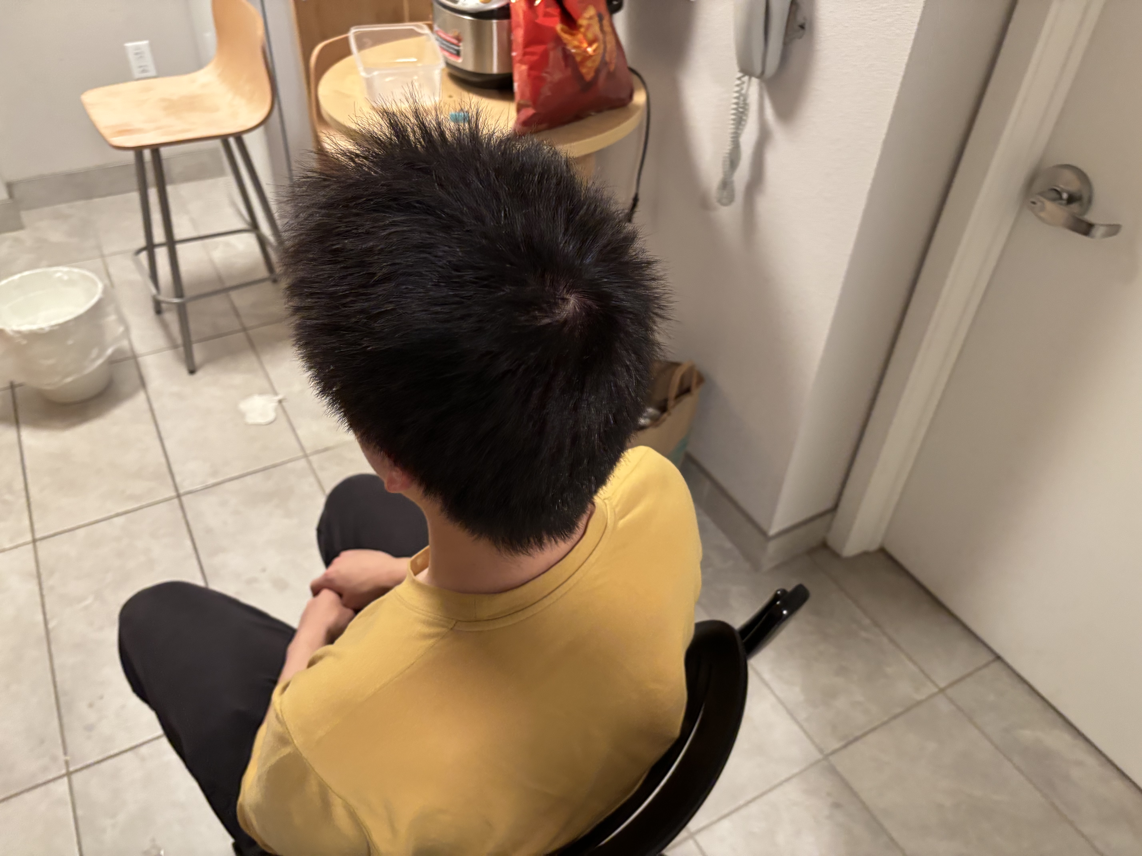
\includegraphics[width=\textwidth]{project-milestone/images/portrait_raw/IMG_0346.png}
            \caption{raw}
        \end{subfigure}
        \hfill
        \begin{subfigure}{0.3\textwidth}
            \centering
            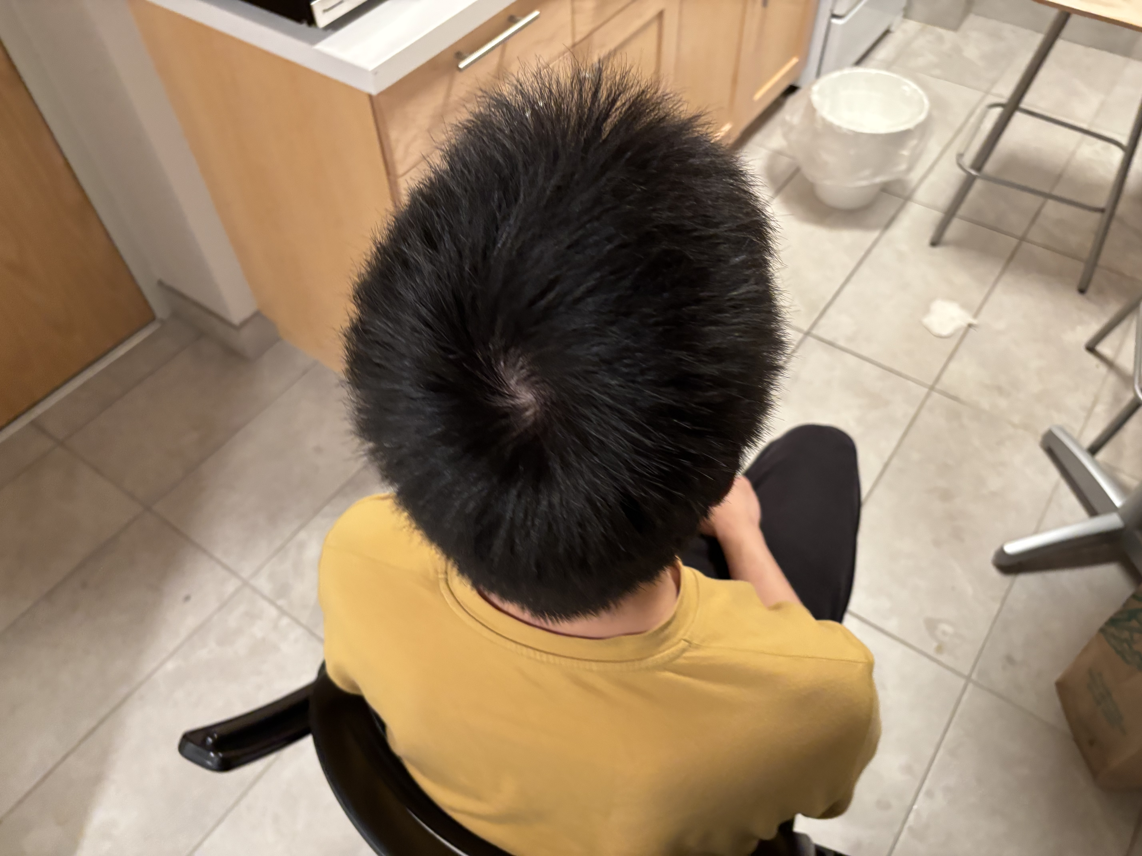
\includegraphics[width=\textwidth]{project-milestone/images/portrait_raw/IMG_0349.png}
            \caption{raw}
        \end{subfigure}
        \vskip\baselineskip
        % second col
        \begin{subfigure}{0.3\textwidth}
            \centering
            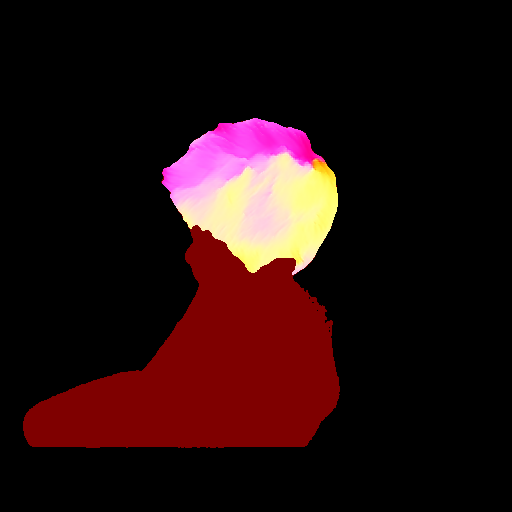
\includegraphics[width=\textwidth]{project-milestone/images/strand_map/IMG_0342.png}
            \caption{processed}
        \end{subfigure}
        \hfill
        \begin{subfigure}{0.3\textwidth}
            \centering
            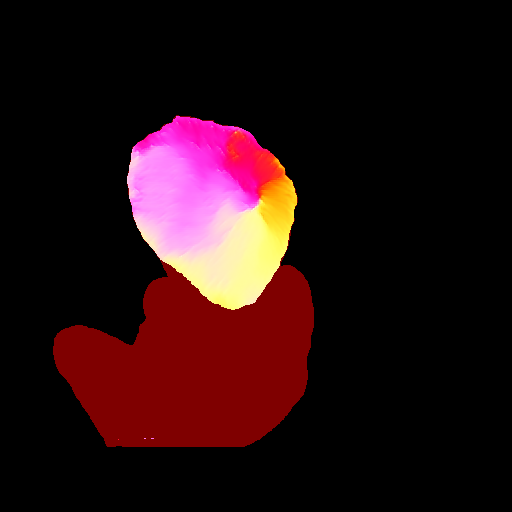
\includegraphics[width=\textwidth]{project-milestone/images/strand_map/IMG_0346.png}
            \caption{processed}
        \end{subfigure}
        \hfill
        \begin{subfigure}{0.3\textwidth}
            \centering
            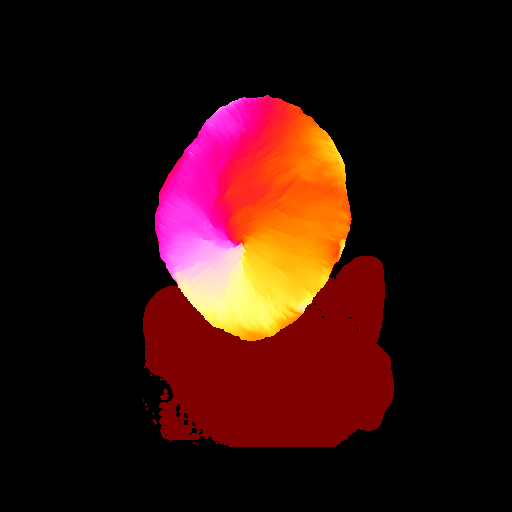
\includegraphics[width=\textwidth]{project-milestone/images/strand_map/IMG_0349.png}
            \caption{processed}
        \end{subfigure}
        
        \caption{Image Preprocessing}
        \label{fig:image_prep}
    \end{figure}

    $\mathbf{Camera:}$ For portrait taken in reality, we use COLMAP, a general-purpose MVS pipeline that processes a set of images to generate a point cloud, to reconstruct the camera position and angle. We also implemented a visualizer for COLMAP for debug purposes. In Figure \ref{fig:colmap_demo}, we see that COLMAP successfully reconstruct camera for the image.
    \begin{figure}[h]
        \centering
        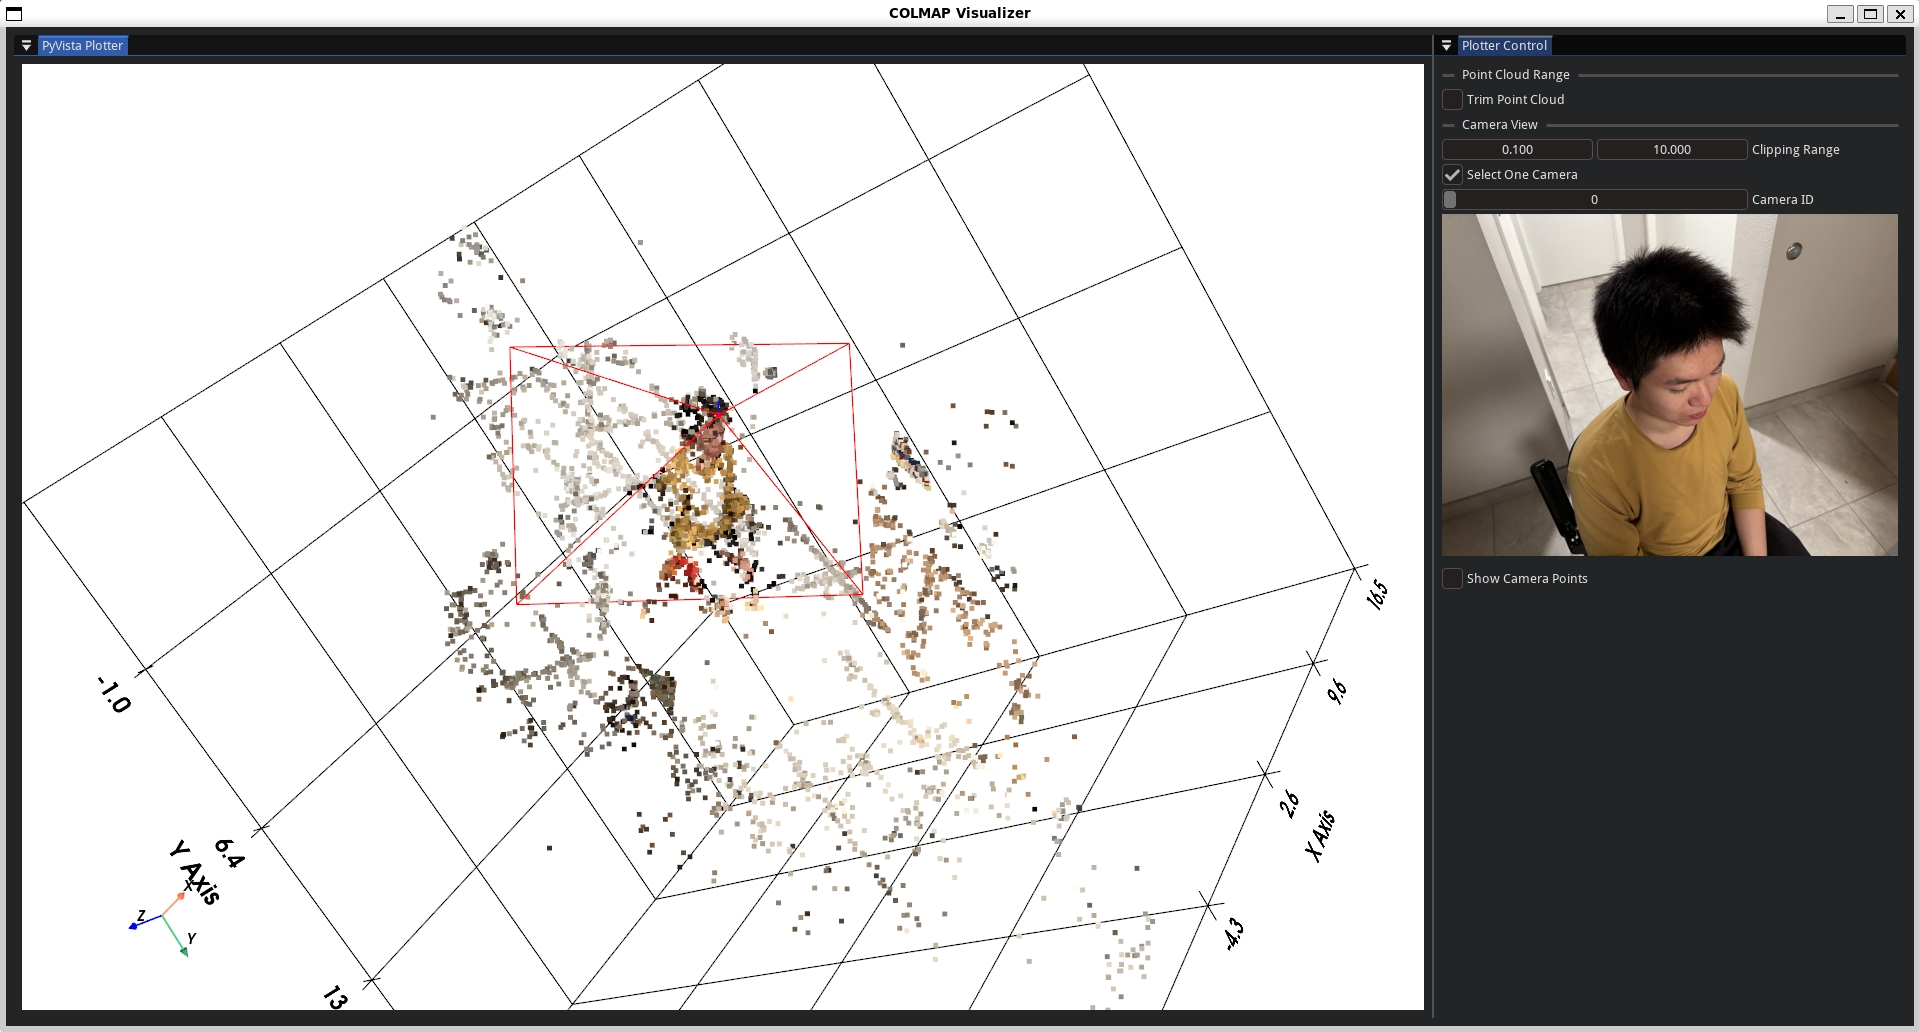
\includegraphics[width=0.5\linewidth]{project-milestone/images/colmap_demo.png}
        \caption{Camera position reconstruction using COLMAP}
        \label{fig:colmap_demo}
    \end{figure}

    \subsection{Neural Orientation Field Model}
    
    The neural orientation field model we proposed consists of multiple MLP layers and residual connections. The input of the network is the spatial coordinates $(x, y, z)$ of the point to be sampled. The output is the normalized orientation of the hair $(\theta, \phi)$, as well as the opacity parameter $\sigma = (\sigma_{void}, \sigma_{hair}, \sigma_{body})$. A softmax layer is used to make $\Vert \sigma \Vert_{2} = 1$.

    \subsection{Volumetric Rendering of a Neural Orientation Field}

    For each camera in the scene, we can emit camera rays for each pixel on the filming plane. Then, hair orientation and occupancy can be sampled along the camera ray. Given the camera view matrix $V \in \mathbb{R}_{4x4}$, the normalized orientation vector in homogeneous coordinate $\mathbf{o} \in \mathbb{R}^{4}$ can be projected to the view space by $\mathbf{o}_{view} = V\mathbf{o}$.

    To project the orientation vectors onto screen space, we need to apply camera projection to the view space vectors. However, as we choose pinhole camera as our camera model, the projected vectors are independent of the camera parameters. In this cases, the screen space projection of the view space orientation is $\mathbf{o}_{screen}$

    \begin{align}
        P &= \begin{bmatrix}
            1 & 0 & 0 & 0 \\
            0 & 1 & 0 & 0 \\
            0 & 0 & 0 & 0 \\
            0 & 0 & 0 & 0
        \end{bmatrix} \\
        \mathbf{o}_{screen} &= P\mathbf{o}_{view}
    \end{align}

    Similar to the volumetric rendering function defined in NeRF \cite{mildenhall_nerf_2020}, our rendering function for screen space orientation can be written as

    \begin{align}
        O(\mathbf{r}) &= \int_{t_{n}}^{t_{f}} T(t) \sigma_{hair}(\mathbf{r}(t)) P V \mathbf{o}(\mathbf{r}(t), \mathbf{d}) dt \\
        T(t) &= exp(-\int_{t_{n}}^{t_{f}} \sigma_{hair}(\mathbf{r}(s)) ds)
    \end{align}

    One important difference between our model and NeRF is we use two separate occupancy for body and hair, while in NeRF one occupancy is used to integrate camera rays. In our case, camera rays can be blocked by face and body that doesn't contribute to the final hair orientation field. These parts are marked red in the preprocessing step s demonstrated in Figure \ref{fig:image_prep}. When training the model, we integrate the 2D hair orientation using the aforementioned volumetric render function. We also run a traditional NeRF volumetric renderer to integrate the body occupancy to generate the body mask. The final loss is defined as the combination of two losses.
    
  \section{Experiment}

  \subsection{DataSet}

  To investigate the convergence behavior of NeRF, we utilized synthetic images generated from Blender, specifically using a scene of Hoover Tower. For hair direction reconstruction, we compiled a dataset of 41 portraits, captured by ourselves, featuring one of our group members.

  \subsection{Metrics}

  The Peak Signal-to-Noise Ratio (PSNR) is a widely used metric in signal processing for assessing image similarity, particularly in image reconstruction tasks. It effectively represents the Mean Squared Error (MSE) between two images in a 2D context.

  \subsection{Baseline}

  We attempted to train a NeRF model to represent hair structure as a radiance field, leveraging it to infer hair orientation. Since NeRF does not inherently encode orientation information, we relied on HairStep to predict orientation. Initial observations showed a slow convergence rate when training on highly detailed scenes, consistent with findings in the original NeRF paper \cite{mildenhall_nerf_2020}, which noted that NeRF tends to capture low-frequency features early in training, see Figure \ref{fig:nerf_slow}. Another consequence of this is that the output of NeRF is often blurred, making HairStep difficult to segment out hair and output reasonable hair direction, thus incapable of holding relevant direction information, see Figure \ref{fig:nerf_base}.
  \begin{figure}[h]
      \centering
      \begin{subfigure}{0.3\textwidth}
            \centering
            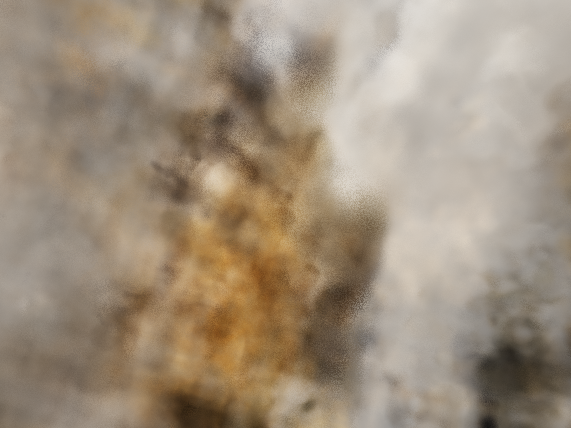
\includegraphics[width=\textwidth]{project-milestone/images/nerf_pred/nerf_800.png}
            \caption{step 800}
        \end{subfigure}
        \hfill
        \begin{subfigure}{0.3\textwidth}
            \centering
            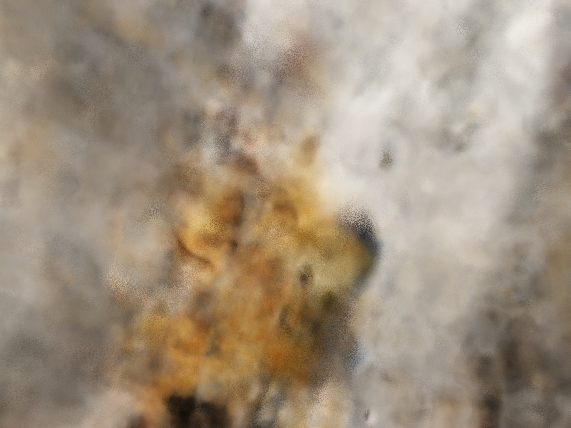
\includegraphics[width=\textwidth]{project-milestone/images/nerf_pred/nerf_4000.png}
            \caption{step 4000}
        \end{subfigure}
        \hfill
        \begin{subfigure}{0.3\textwidth}
            \centering
            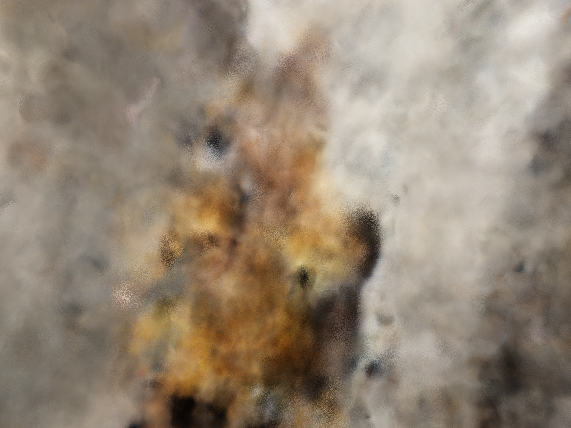
\includegraphics[width=\textwidth]{project-milestone/images/nerf_pred/nerf_10000.png}
            \caption{step 10000}
        \end{subfigure}
        
      \caption{NeRF's output on evaluation set, shows slow convergence and high variance}
      \label{fig:nerf_slow}
  \end{figure}

  We also observed signs of overfitting in NeRF, with the PSNR on the evaluation set stabilizing around 1000 batches. We aim to address this with regularization methods (WIP). Additionally, we hypothesize that the model may converge faster on a smaller dataset, given that the hair orientation field we aim to fit is view-independent and should not vary with camera position. As the outcome is evident, we opted not to measure PSNR for the NeRF baseline.

  %% We tried to train a NeRF model to reconstruct hair structure as a radiance field, and use it to predict hair orientation.
  %% NeRF doesn't include the latent orientation data. Therefore, we must still predict the orientation with HairStep.
  %% We observed low convergence rate when trained on highly detailed scene. Cite original NeRF paper (NeRF tend to learn low frequency function in the early stage). (add figure show slow convergence)
  %% We observed overfitting on NeRF. PSNR on the evaluation set stop increasing at around 1000 batches. (WIP) we'll try to solve this problem by regularization.
  %% (WIP) We suspect our model will converge faster on smaller dataset: The orientation field we are trying to fit is view independent (the hair orientation we sampled from multiple direction does not vary based on the camera position).
  %% No need to measure PSNR on the NeRF baseline, as the result is obvious.

  \begin{figure}[h]
        \centering
        \begin{subfigure}{0.3\textwidth}
            \centering
            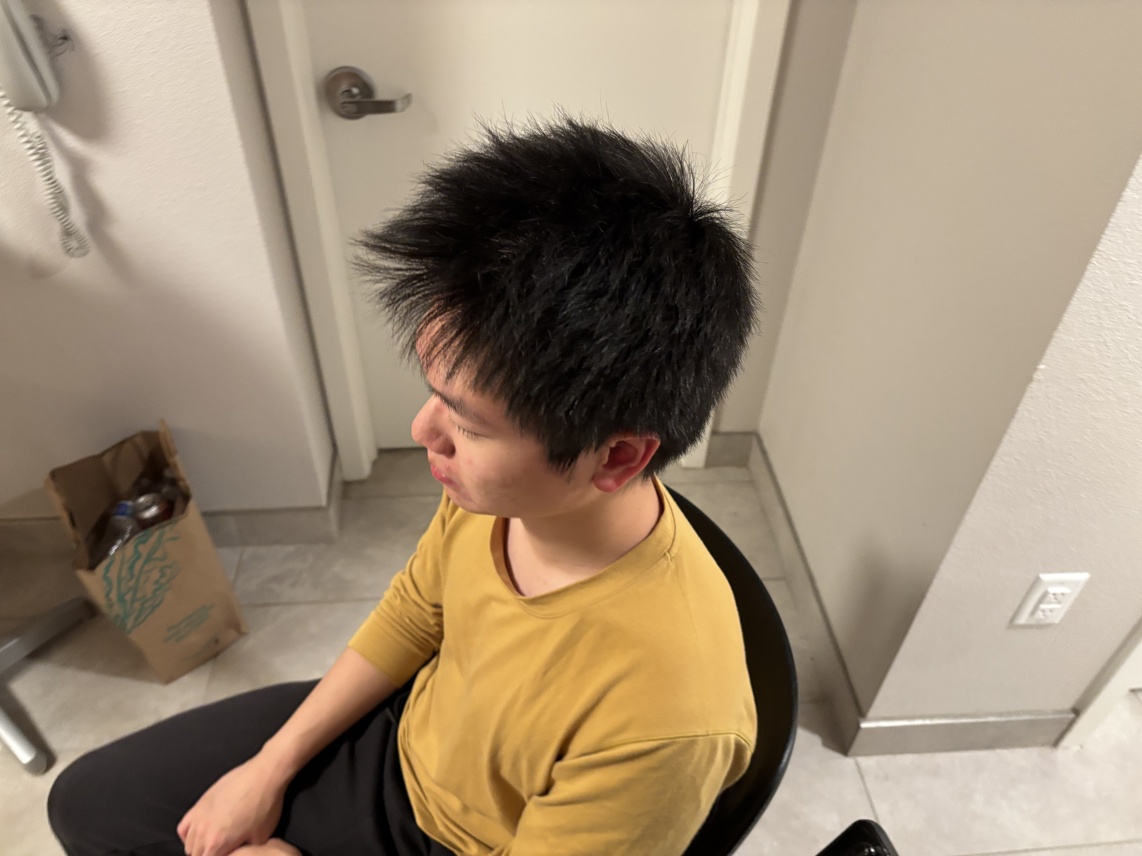
\includegraphics[width=\textwidth]{project-milestone/images/portrait_raw/IMG_0342.png}
            \caption{raw}
        \end{subfigure}
        \quad
        \begin{subfigure}{0.3\textwidth}
            \centering
            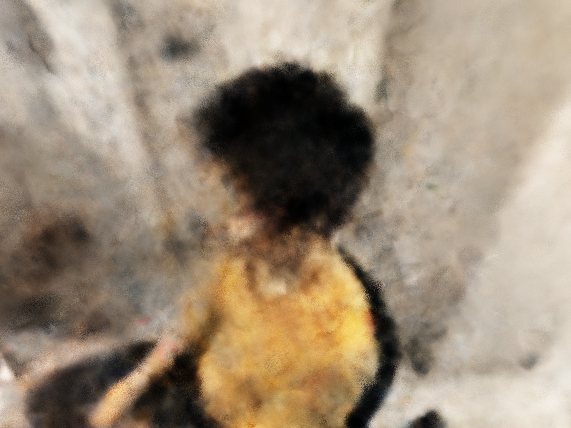
\includegraphics[width=\textwidth]{project-milestone/images/nerf_pred/31.png}
            \caption{NeRF output}
        \end{subfigure}

        \vskip\baselineskip
        \begin{subfigure}{0.3\textwidth}
            \centering
            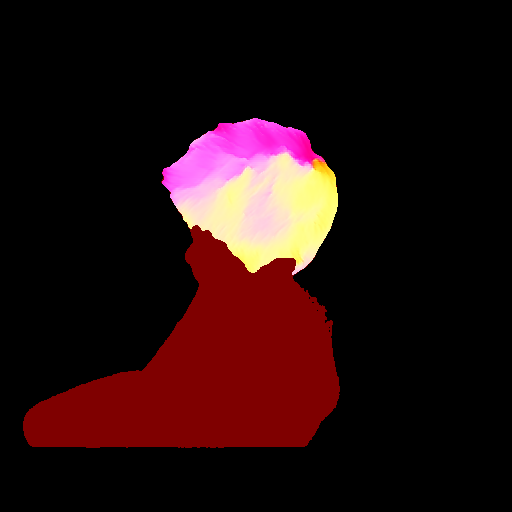
\includegraphics[width=\textwidth]{project-milestone/images/strand_map/IMG_0342.png}
            \caption{hair direction extraction ground truth}
        \end{subfigure}
        \quad
        \begin{subfigure}{0.3\textwidth}
            \centering
            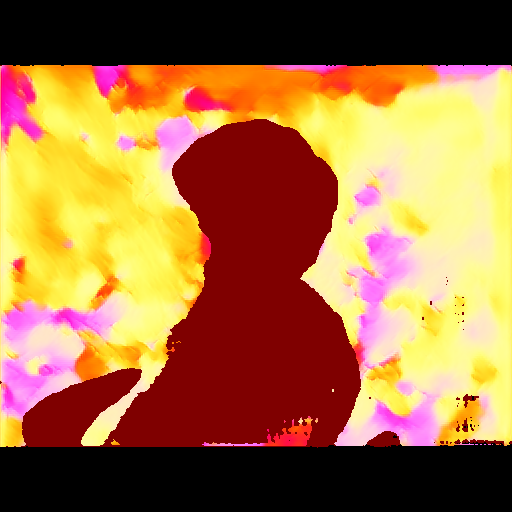
\includegraphics[width=\textwidth]{project-milestone/images/nerf_pred_strand/31.png}
            \caption{hair direction extraction from NeRF output}
        \end{subfigure}

        \caption{Baseline Experiment}
        \label{fig:nerf_base}
  \end{figure}

  \section{Contribution}

  \subsection{Fangjun Zhou}

  Wrote preprocessing script that uses COLMAP to extract features and camera poses. Wrote colmap\_visualizer using imagui and pyvista to help visualize the extracted point cloud / camera position. Wrote helper methods to construct camera rays for NeRF training. Rendered hoover tower dataset in Blender. Implement and trained NeRF baseline. Derive orientation vector projection volumetric render function. Wrote method section in the milestone report.

  \subsection{Weiran Xu}
  
  Contributed to building the human portrait dataset and applied HairStep for image preprocessing and hair strand direction extraction, preparing the data for analysis. Also wrote part of experiment section in the milestone report, detailing methodology and preliminary findings.

  \subsection{Zhenyu Zhang}
  
  Responsible for refactoring Tiny NeRF, do the training and testing related to Tiny NeRF, and implementing the code for 3D vector field reconstruction of hair growth. This included model code, loss computation code, camera view transformation and coordinate system conversion code, as well as the code of calculations for remapping 3D vectors in space to the camera frame.
  
  % Intended experiment
  \section{Work in Progress}

  We've finish implementing our proposed model but haven't start the experiment. We're also planning to add more baselines to compare with. On top of that, the current model is slow to converge. We're planning to implement hierarchical volume sampling mentioned in the original NeRF paper to speed up convergence.

  \printbibliography

\end{document}
